% =====================================================================
\section{Object Construction}\label{sec:construction}
A composite object is a small scene graph. Leaves draw one primitive with their own $S,R,T$; group nodes only carry
a transform and a name. Every node has a name, an object, a purpose and, if it moves, an \code{animation} text;
the Excel workbook lists them all (the exporter writes \code{build/scene\_export.json}). Table~\ref{tab:parts} is
generated from that file: the scene holds \nLeaves{} leaf parts in 14 export objects. Test T38 checks that every
leaf is a cube, sphere, cylinder or cone, and T70/T67/T96/T99 check each new object for ``lab primitives only,
every node named''.

\begin{table}[h]
\centering\small
\caption{Parts per composite object, generated from \code{build/scene\_export.json}. Depth is the deepest group
level. The \emph{Target Rover} row counts all three intruders (\partsRover{} parts each). Base, bunker and
environment counts are the values at the time of the last export; they grow when engineers add detail, and
the table is regenerated by \code{report/gen\_tables.py}.}
\label{tab:parts}
% generated by report/gen_tables.py from build/scene_export.json -- do not edit
\begin{tabular}{@{}lrrrp{4.6cm}l@{}}
\toprule
Object (export name) & Parts & Groups & Depth & Cube / Sphere / Cylinder / Cone / Frustum & Shading\\\midrule
Terrain & 1 & 1 & 1 & 1 height-field disc & Gouraud 1\\
Backdrop & 120 & 47 & 3 & 0 / 24 / 10 / 86 / 0 & Gouraud 120\\
Environment & 651 & 89 & 3 & 46 / 201 / 237 / 167 / 0 & Gouraud 651\\
Command Bunker & 363 & 16 & 3 & 264 / 19 / 80 / 0 / 0 & Flat 363\\
Autonomous UAV & 67 & 17 & 3 & 32 / 9 / 21 / 4 / 1 & Phong 66,\allowbreak{} Additive beam 1\\
Base & 1168 & 36 & 3 & 504 / 31 / 633 / 0 / 0 & Flat 626,\allowbreak{} Gouraud 542\\
Target Rover & 78 & 6 & 2 & 18 / 36 / 24 / 0 / 0 & Phong 78\\
Main Battle Tank & 226 & 29 & 5 & 154 / 4 / 68 / 0 / 0 & Phong 226\\
Scout Helicopter & 68 & 19 & 7 & 29 / 10 / 27 / 1 / 1 & Phong 67,\allowbreak{} Additive beam 1\\
AA Gatling Gun & 57 & 5 & 4 & 12 / 3 / 42 / 0 / 0 & Phong 57\\
Air-defence radar & 102 & 4 & 4 & 60 / 2 / 39 / 1 / 0 & Phong 102\\
Boom barrier & 20 & 2 & 2 & 17 / 2 / 1 / 0 / 0 & Gouraud 20\\
Windsock & 15 & 7 & 7 & 1 / 0 / 14 / 0 / 0 & Gouraud 15\\
Flag & 47 & 14 & 14 & 40 / 2 / 5 / 0 / 0 & Gouraud 47\\
\midrule
Total & 2983 & 292 & & &\\
\bottomrule
\end{tabular}

\end{table}

\noindent All hierarchy diagrams below are generated from the same export: \emph{[n]} is the number of leaf
parts below a node, ``$\times k$'' collapses $k$ identical sibling groups, and italic lines summarise the leaf
parts that hang directly under a group.

% ---------------------------------------------------------------------
\subsection{Underground command bunker}
The v1 surface block was replaced by an \emph{underground} bunker (\partsBunker{} parts, Flat shading). An open
entrance trench (retaining walls, guard rails, cage lamps) follows the vehicle track down a 7\,m ramp
($z=13\to6$, 1.5\,m half-width) to the blast-door plane at $z=4$; behind it a tunnel leads to the command and
information centre (CIC), a bunk room, a generator room and an emergency exit shaft with a ladder up to a surface
hatch. All rooms share the floor level $y=-3.4$\,m, the ceiling is at $-0.8$\,m (2.6\,m clear height) and the
terrain stays at least 0.15\,m above the roof slab (T60). On the surface only vent stacks with spinning fans, the
beacon mast (the point light L1), antennas, the hatch and a few sandbags remain. The CIC contains consoles whose
screens use the procedural \emph{Screen} surface (map grid, radar sweep, text bars). The two door leaves
(\emph{Door leaf W/E}, 6 parts each, plus two \emph{Beacon spinners}) are the animated part of the bunker and
are described in Section~\ref{sec:control}.

\begin{figure}[h]
\centering
\begin{minipage}[t]{0.52\linewidth}\vspace{0pt}% generated by report/gen_tables.py from build/scene_export.json -- do not edit
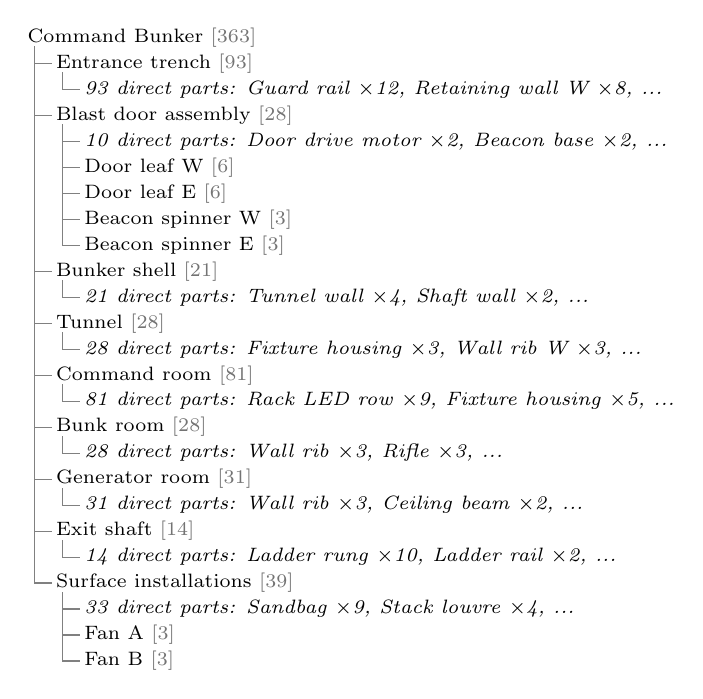
\begin{tikzpicture}[x=0.36cm,y=-0.33cm,font=\scriptsize]
\node[anchor=west,inner sep=0pt] (n0) at (0,0) {Command Bunker \textcolor{black!55}{[363]}};
\node[anchor=west,inner sep=0pt] (n1) at (1,1) {Entrance trench \textcolor{black!55}{[93]}};
\draw[black!50,thin] (0.25,0.35) |- (0.88,1);
\node[anchor=west,inner sep=0pt] (n2) at (2,2) {\textit{93 direct parts: Guard rail $\times$12, Retaining wall W $\times$8, ...}};
\draw[black!50,thin] (1.25,1.35) |- (1.88,2);
\node[anchor=west,inner sep=0pt] (n3) at (1,3) {Blast door assembly \textcolor{black!55}{[28]}};
\draw[black!50,thin] (0.25,0.35) |- (0.88,3);
\node[anchor=west,inner sep=0pt] (n4) at (2,4) {\textit{10 direct parts: Door drive motor $\times$2, Beacon base $\times$2, ...}};
\draw[black!50,thin] (1.25,3.35) |- (1.88,4);
\node[anchor=west,inner sep=0pt] (n5) at (2,5) {Door leaf W \textcolor{black!55}{[6]}};
\draw[black!50,thin] (1.25,3.35) |- (1.88,5);
\node[anchor=west,inner sep=0pt] (n6) at (2,6) {Door leaf E \textcolor{black!55}{[6]}};
\draw[black!50,thin] (1.25,3.35) |- (1.88,6);
\node[anchor=west,inner sep=0pt] (n7) at (2,7) {Beacon spinner W \textcolor{black!55}{[3]}};
\draw[black!50,thin] (1.25,3.35) |- (1.88,7);
\node[anchor=west,inner sep=0pt] (n8) at (2,8) {Beacon spinner E \textcolor{black!55}{[3]}};
\draw[black!50,thin] (1.25,3.35) |- (1.88,8);
\node[anchor=west,inner sep=0pt] (n9) at (1,9) {Bunker shell \textcolor{black!55}{[21]}};
\draw[black!50,thin] (0.25,0.35) |- (0.88,9);
\node[anchor=west,inner sep=0pt] (n10) at (2,10) {\textit{21 direct parts: Tunnel wall $\times$4, Shaft wall $\times$2, ...}};
\draw[black!50,thin] (1.25,9.35) |- (1.88,10);
\node[anchor=west,inner sep=0pt] (n11) at (1,11) {Tunnel \textcolor{black!55}{[28]}};
\draw[black!50,thin] (0.25,0.35) |- (0.88,11);
\node[anchor=west,inner sep=0pt] (n12) at (2,12) {\textit{28 direct parts: Fixture housing $\times$3, Wall rib W $\times$3, ...}};
\draw[black!50,thin] (1.25,11.35) |- (1.88,12);
\node[anchor=west,inner sep=0pt] (n13) at (1,13) {Command room \textcolor{black!55}{[81]}};
\draw[black!50,thin] (0.25,0.35) |- (0.88,13);
\node[anchor=west,inner sep=0pt] (n14) at (2,14) {\textit{81 direct parts: Rack LED row $\times$9, Fixture housing $\times$5, ...}};
\draw[black!50,thin] (1.25,13.35) |- (1.88,14);
\node[anchor=west,inner sep=0pt] (n15) at (1,15) {Bunk room \textcolor{black!55}{[28]}};
\draw[black!50,thin] (0.25,0.35) |- (0.88,15);
\node[anchor=west,inner sep=0pt] (n16) at (2,16) {\textit{28 direct parts: Wall rib $\times$3, Rifle $\times$3, ...}};
\draw[black!50,thin] (1.25,15.35) |- (1.88,16);
\node[anchor=west,inner sep=0pt] (n17) at (1,17) {Generator room \textcolor{black!55}{[31]}};
\draw[black!50,thin] (0.25,0.35) |- (0.88,17);
\node[anchor=west,inner sep=0pt] (n18) at (2,18) {\textit{31 direct parts: Wall rib $\times$3, Ceiling beam $\times$2, ...}};
\draw[black!50,thin] (1.25,17.35) |- (1.88,18);
\node[anchor=west,inner sep=0pt] (n19) at (1,19) {Exit shaft \textcolor{black!55}{[14]}};
\draw[black!50,thin] (0.25,0.35) |- (0.88,19);
\node[anchor=west,inner sep=0pt] (n20) at (2,20) {\textit{14 direct parts: Ladder rung $\times$10, Ladder rail $\times$2, ...}};
\draw[black!50,thin] (1.25,19.35) |- (1.88,20);
\node[anchor=west,inner sep=0pt] (n21) at (1,21) {Surface installations \textcolor{black!55}{[39]}};
\draw[black!50,thin] (0.25,0.35) |- (0.88,21);
\node[anchor=west,inner sep=0pt] (n22) at (2,22) {\textit{33 direct parts: Sandbag $\times$9, Stack louvre $\times$4, ...}};
\draw[black!50,thin] (1.25,21.35) |- (1.88,22);
\node[anchor=west,inner sep=0pt] (n23) at (2,23) {Fan A \textcolor{black!55}{[3]}};
\draw[black!50,thin] (1.25,21.35) |- (1.88,23);
\node[anchor=west,inner sep=0pt] (n24) at (2,24) {Fan B \textcolor{black!55}{[3]}};
\draw[black!50,thin] (1.25,21.35) |- (1.88,24);
\end{tikzpicture}
\end{minipage}\hfill
\begin{minipage}[t]{0.44\linewidth}\vspace{0pt}
\footnotesize
\begin{tabular}{@{}ll@{}}\toprule
Floor/ceiling & $-3.4$\,m / $-0.8$\,m\\
Ramp & $z$ 13 $\to$ 6, 3\,m wide\\
Door plane & $z=4$, opening $2.6\times2.6$\,m\\
Footprint & $x\in[-5.5,5.5]$, $z\in[-8.5,4]$\\
Walk floors / walls & 12 / 36 boxes (T69)\\
Indoor volumes & 5 (T69)\\
Shading & Flat, all leaves (T67)\\\bottomrule
\end{tabular}
\end{minipage}
\caption{Bunker hierarchy (from the export) and key dimensions (\code{BaseLayout.h}, T67--T69).}
\label{fig:tree-bunker}
\end{figure}

% ---------------------------------------------------------------------
\subsection{The base apron}
The apron (r $\approx$ 20--36\,m) is built by \code{Base.cpp}: \partsBase{} static parts (Flat/Gouraud) plus the three animated
objects of Section~\ref{sec:control}. It contains a HESCO bastion perimeter (204 cells with upper tiers) with
concertina wire coils, four guard towers at $r=32.4$\,m, an outer gate with booth, jersey barriers and tank traps,
an asphalt road with painted lines, the helipad (disc, ``H'', a 24-mark circle, 16 blue edge lights and three
practical lights), a motor pool (four containers, two trucks, a camouflage-net bay and the tank spot), a fuel depot
(dike, two bladders, pump, light tower), three Quonset barracks, and the sand-bag ring and fence around the AA-gun
and radar pads. Test T72 checks that the wall is closed except for one 9--11\,m gate gap; T71 that no part
intersects the pads that other objects occupy; T77 that nothing is an occluder and every part lies inside $r=36$\,m.

\begin{figure}[h]
\centering
\begin{minipage}[t]{0.56\linewidth}\vspace{0pt}% generated by report/gen_tables.py from build/scene_export.json -- do not edit
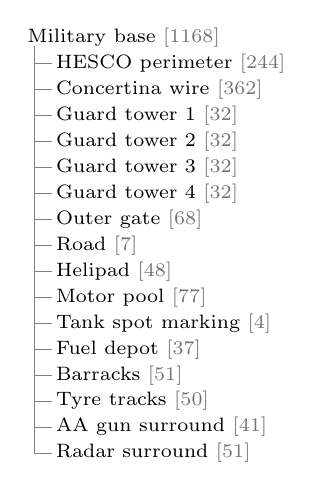
\begin{tikzpicture}[x=0.36cm,y=-0.33cm,font=\scriptsize]
\node[anchor=west,inner sep=0pt] (n0) at (0,0) {Military base \textcolor{black!55}{[1168]}};
\node[anchor=west,inner sep=0pt] (n1) at (1,1) {HESCO perimeter \textcolor{black!55}{[244]}};
\draw[black!50,thin] (0.25,0.35) |- (0.88,1);
\node[anchor=west,inner sep=0pt] (n2) at (1,2) {Concertina wire \textcolor{black!55}{[362]}};
\draw[black!50,thin] (0.25,0.35) |- (0.88,2);
\node[anchor=west,inner sep=0pt] (n3) at (1,3) {Guard tower 1 \textcolor{black!55}{[32]}};
\draw[black!50,thin] (0.25,0.35) |- (0.88,3);
\node[anchor=west,inner sep=0pt] (n4) at (1,4) {Guard tower 2 \textcolor{black!55}{[32]}};
\draw[black!50,thin] (0.25,0.35) |- (0.88,4);
\node[anchor=west,inner sep=0pt] (n5) at (1,5) {Guard tower 3 \textcolor{black!55}{[32]}};
\draw[black!50,thin] (0.25,0.35) |- (0.88,5);
\node[anchor=west,inner sep=0pt] (n6) at (1,6) {Guard tower 4 \textcolor{black!55}{[32]}};
\draw[black!50,thin] (0.25,0.35) |- (0.88,6);
\node[anchor=west,inner sep=0pt] (n7) at (1,7) {Outer gate \textcolor{black!55}{[68]}};
\draw[black!50,thin] (0.25,0.35) |- (0.88,7);
\node[anchor=west,inner sep=0pt] (n8) at (1,8) {Road \textcolor{black!55}{[7]}};
\draw[black!50,thin] (0.25,0.35) |- (0.88,8);
\node[anchor=west,inner sep=0pt] (n9) at (1,9) {Helipad \textcolor{black!55}{[48]}};
\draw[black!50,thin] (0.25,0.35) |- (0.88,9);
\node[anchor=west,inner sep=0pt] (n10) at (1,10) {Motor pool \textcolor{black!55}{[77]}};
\draw[black!50,thin] (0.25,0.35) |- (0.88,10);
\node[anchor=west,inner sep=0pt] (n11) at (1,11) {Tank spot marking \textcolor{black!55}{[4]}};
\draw[black!50,thin] (0.25,0.35) |- (0.88,11);
\node[anchor=west,inner sep=0pt] (n12) at (1,12) {Fuel depot \textcolor{black!55}{[37]}};
\draw[black!50,thin] (0.25,0.35) |- (0.88,12);
\node[anchor=west,inner sep=0pt] (n13) at (1,13) {Barracks \textcolor{black!55}{[51]}};
\draw[black!50,thin] (0.25,0.35) |- (0.88,13);
\node[anchor=west,inner sep=0pt] (n14) at (1,14) {Tyre tracks \textcolor{black!55}{[50]}};
\draw[black!50,thin] (0.25,0.35) |- (0.88,14);
\node[anchor=west,inner sep=0pt] (n15) at (1,15) {AA gun surround \textcolor{black!55}{[41]}};
\draw[black!50,thin] (0.25,0.35) |- (0.88,15);
\node[anchor=west,inner sep=0pt] (n16) at (1,16) {Radar surround \textcolor{black!55}{[51]}};
\draw[black!50,thin] (0.25,0.35) |- (0.88,16);
\end{tikzpicture}
\end{minipage}\hfill
\begin{minipage}[t]{0.40\linewidth}\vspace{0pt}
\captionsetup{type=figure}
\pic{figures_v4/base_gate}{\linewidth}
\end{minipage}
\caption{Base hierarchy (left, from the export; the figure ``base\_gate'' (right) shows the outer gate with boom
barrier, booth and towers).}
\end{figure}

% ---------------------------------------------------------------------
\subsection{UAV with launcher rails}
The quadcopter (\partsUav{} parts, Phong) has a fuselage, canopy, four motor mounts with rotors, landing gear, strobe and
navigation LEDs, and the two-axis searchlight gimbal
\emph{body $\to$ gimbal yaw $\to$ gimbal pitch $\to$ \{lamp, lens, thermal camera, light frustum\}} that the thermal
tracker and the searchlight share. v4 adds two \emph{launcher rails} under the fuselage (14 parts each); each rail
carries two missiles built from a cylinder body, a cone nose and four fins (6 parts). A round is hidden when it is launched and
reappears after the 10\,s reload (Section~\ref{sec:game}). The rotor-blur discs are translucent cylinders
($\alpha<1$, drawn in a separate pass, no shadow).


% ---------------------------------------------------------------------
\subsection{Intruder rover}
Each of the three intruders is a six-wheeled UGV with \partsRover{} parts: cube chassis, hull and motor box; six
cylinder wheels (axis turned onto $x$ by $R_y(90^\circ)$, spin $=R_z$); sphere hubs; five IR line sensors; a rotating
scanner on a pivot. The hottest part is the motor box (thermal value 0.97), which is what the UAV's tracker locks on.
The three rovers share the geometry and have distinct part ids (\code{ROV-07}, \code{ROV2-07}, \code{ROV3-07}).
When a rover is destroyed its parts become rigid debris (Section~\ref{sec:game}).


% ---------------------------------------------------------------------
\subsection{Main battle tank with 80 animated track links}
The tank (\partsTank{} parts, Phong, scale about 0.8 of a Leopard/M1 class machine) parks at the motor pool facing the road.
Its hull carries plates, skirts, an exhaust grille, lights and antennas; the turret carries cheeks, a bustle,
sights, a commander's cupola with a rotating machine gun and smoke launchers; the gun is
\emph{gun pitch $\to$ barrel recoil $\to$ barrel, fume extractor, muzzle brake}. Each track is a group of
$40$ link cubes ($\nTrackLinks$ in total) plus seven road wheels, a drive sprocket, an idler and return rollers. The link
cubes are not rigidly modelled: each frame their transform is set from the arc length along a closed stadium-shaped
path (Section~\ref{sec:control}). Test T80 checks that all 80 links stay on the path (max distance $0$\,m).


\begin{figure}[h]
\centering
\begin{minipage}[t]{0.31\linewidth}\vspace{0pt}% generated by report/gen_tables.py from build/scene_export.json -- do not edit
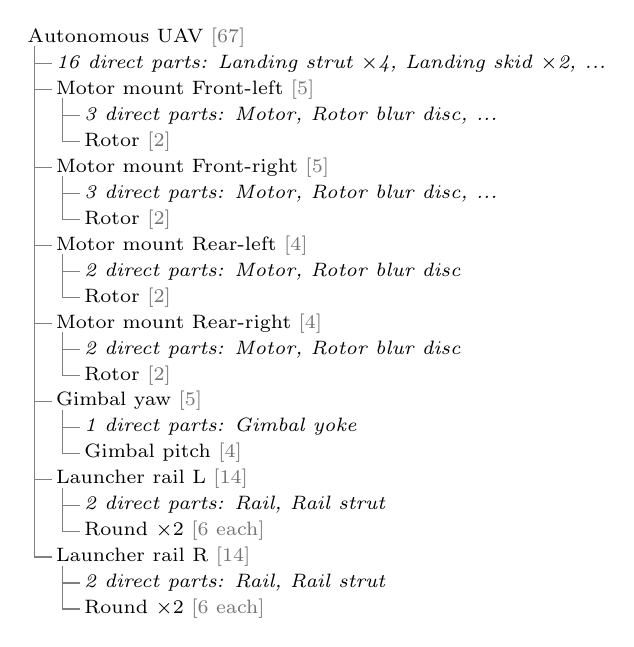
\begin{tikzpicture}[x=0.36cm,y=-0.33cm,font=\scriptsize]
\node[anchor=west,inner sep=0pt] (n0) at (0,0) {Autonomous UAV \textcolor{black!55}{[67]}};
\node[anchor=west,inner sep=0pt] (n1) at (1,1) {\textit{16 direct parts: Landing strut $\times$4, Landing skid $\times$2, ...}};
\draw[black!50,thin] (0.25,0.35) |- (0.88,1);
\node[anchor=west,inner sep=0pt] (n2) at (1,2) {Motor mount Front-left \textcolor{black!55}{[5]}};
\draw[black!50,thin] (0.25,0.35) |- (0.88,2);
\node[anchor=west,inner sep=0pt] (n3) at (2,3) {\textit{3 direct parts: Motor, Rotor blur disc, ...}};
\draw[black!50,thin] (1.25,2.35) |- (1.88,3);
\node[anchor=west,inner sep=0pt] (n4) at (2,4) {Rotor \textcolor{black!55}{[2]}};
\draw[black!50,thin] (1.25,2.35) |- (1.88,4);
\node[anchor=west,inner sep=0pt] (n5) at (1,5) {Motor mount Front-right \textcolor{black!55}{[5]}};
\draw[black!50,thin] (0.25,0.35) |- (0.88,5);
\node[anchor=west,inner sep=0pt] (n6) at (2,6) {\textit{3 direct parts: Motor, Rotor blur disc, ...}};
\draw[black!50,thin] (1.25,5.35) |- (1.88,6);
\node[anchor=west,inner sep=0pt] (n7) at (2,7) {Rotor \textcolor{black!55}{[2]}};
\draw[black!50,thin] (1.25,5.35) |- (1.88,7);
\node[anchor=west,inner sep=0pt] (n8) at (1,8) {Motor mount Rear-left \textcolor{black!55}{[4]}};
\draw[black!50,thin] (0.25,0.35) |- (0.88,8);
\node[anchor=west,inner sep=0pt] (n9) at (2,9) {\textit{2 direct parts: Motor, Rotor blur disc}};
\draw[black!50,thin] (1.25,8.35) |- (1.88,9);
\node[anchor=west,inner sep=0pt] (n10) at (2,10) {Rotor \textcolor{black!55}{[2]}};
\draw[black!50,thin] (1.25,8.35) |- (1.88,10);
\node[anchor=west,inner sep=0pt] (n11) at (1,11) {Motor mount Rear-right \textcolor{black!55}{[4]}};
\draw[black!50,thin] (0.25,0.35) |- (0.88,11);
\node[anchor=west,inner sep=0pt] (n12) at (2,12) {\textit{2 direct parts: Motor, Rotor blur disc}};
\draw[black!50,thin] (1.25,11.35) |- (1.88,12);
\node[anchor=west,inner sep=0pt] (n13) at (2,13) {Rotor \textcolor{black!55}{[2]}};
\draw[black!50,thin] (1.25,11.35) |- (1.88,13);
\node[anchor=west,inner sep=0pt] (n14) at (1,14) {Gimbal yaw \textcolor{black!55}{[5]}};
\draw[black!50,thin] (0.25,0.35) |- (0.88,14);
\node[anchor=west,inner sep=0pt] (n15) at (2,15) {\textit{1 direct parts: Gimbal yoke}};
\draw[black!50,thin] (1.25,14.35) |- (1.88,15);
\node[anchor=west,inner sep=0pt] (n16) at (2,16) {Gimbal pitch \textcolor{black!55}{[4]}};
\draw[black!50,thin] (1.25,14.35) |- (1.88,16);
\node[anchor=west,inner sep=0pt] (n17) at (1,17) {Launcher rail L \textcolor{black!55}{[14]}};
\draw[black!50,thin] (0.25,0.35) |- (0.88,17);
\node[anchor=west,inner sep=0pt] (n18) at (2,18) {\textit{2 direct parts: Rail, Rail strut}};
\draw[black!50,thin] (1.25,17.35) |- (1.88,18);
\node[anchor=west,inner sep=0pt] (n19) at (2,19) {Round $\times$2 \textcolor{black!55}{[6 each]}};
\draw[black!50,thin] (1.25,17.35) |- (1.88,19);
\node[anchor=west,inner sep=0pt] (n20) at (1,20) {Launcher rail R \textcolor{black!55}{[14]}};
\draw[black!50,thin] (0.25,0.35) |- (0.88,20);
\node[anchor=west,inner sep=0pt] (n21) at (2,21) {\textit{2 direct parts: Rail, Rail strut}};
\draw[black!50,thin] (1.25,20.35) |- (1.88,21);
\node[anchor=west,inner sep=0pt] (n22) at (2,22) {Round $\times$2 \textcolor{black!55}{[6 each]}};
\draw[black!50,thin] (1.25,20.35) |- (1.88,22);
\end{tikzpicture}
\end{minipage}\hfill
\begin{minipage}[t]{0.31\linewidth}\vspace{0pt}% generated by report/gen_tables.py from build/scene_export.json -- do not edit
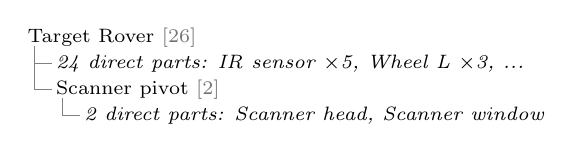
\begin{tikzpicture}[x=0.36cm,y=-0.33cm,font=\scriptsize]
\node[anchor=west,inner sep=0pt] (n0) at (0,0) {Target Rover \textcolor{black!55}{[26]}};
\node[anchor=west,inner sep=0pt] (n1) at (1,1) {\textit{24 direct parts: IR sensor $\times$5, Wheel L $\times$3, ...}};
\draw[black!50,thin] (0.25,0.35) |- (0.88,1);
\node[anchor=west,inner sep=0pt] (n2) at (1,2) {Scanner pivot \textcolor{black!55}{[2]}};
\draw[black!50,thin] (0.25,0.35) |- (0.88,2);
\node[anchor=west,inner sep=0pt] (n3) at (2,3) {\textit{2 direct parts: Scanner head, Scanner window}};
\draw[black!50,thin] (1.25,2.35) |- (1.88,3);
\end{tikzpicture}
\end{minipage}\hfill
\begin{minipage}[t]{0.35\linewidth}\vspace{0pt}% generated by report/gen_tables.py from build/scene_export.json -- do not edit
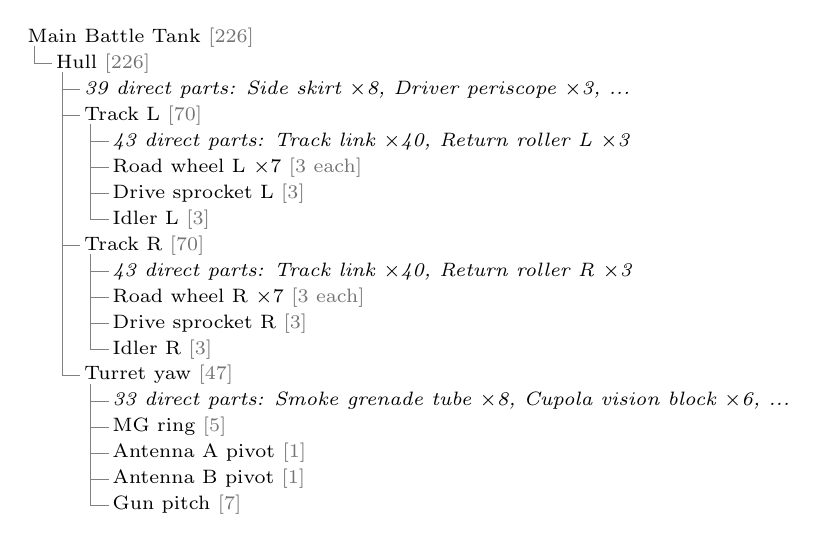
\begin{tikzpicture}[x=0.36cm,y=-0.33cm,font=\scriptsize]
\node[anchor=west,inner sep=0pt] (n0) at (0,0) {Main Battle Tank \textcolor{black!55}{[226]}};
\node[anchor=west,inner sep=0pt] (n1) at (1,1) {Hull \textcolor{black!55}{[226]}};
\draw[black!50,thin] (0.25,0.35) |- (0.88,1);
\node[anchor=west,inner sep=0pt] (n2) at (2,2) {\textit{39 direct parts: Side skirt $\times$8, Driver periscope $\times$3, ...}};
\draw[black!50,thin] (1.25,1.35) |- (1.88,2);
\node[anchor=west,inner sep=0pt] (n3) at (2,3) {Track L \textcolor{black!55}{[70]}};
\draw[black!50,thin] (1.25,1.35) |- (1.88,3);
\node[anchor=west,inner sep=0pt] (n4) at (3,4) {\textit{43 direct parts: Track link $\times$40, Return roller L $\times$3}};
\draw[black!50,thin] (2.25,3.35) |- (2.88,4);
\node[anchor=west,inner sep=0pt] (n5) at (3,5) {Road wheel L $\times$7 \textcolor{black!55}{[3 each]}};
\draw[black!50,thin] (2.25,3.35) |- (2.88,5);
\node[anchor=west,inner sep=0pt] (n6) at (3,6) {Drive sprocket L \textcolor{black!55}{[3]}};
\draw[black!50,thin] (2.25,3.35) |- (2.88,6);
\node[anchor=west,inner sep=0pt] (n7) at (3,7) {Idler L \textcolor{black!55}{[3]}};
\draw[black!50,thin] (2.25,3.35) |- (2.88,7);
\node[anchor=west,inner sep=0pt] (n8) at (2,8) {Track R \textcolor{black!55}{[70]}};
\draw[black!50,thin] (1.25,1.35) |- (1.88,8);
\node[anchor=west,inner sep=0pt] (n9) at (3,9) {\textit{43 direct parts: Track link $\times$40, Return roller R $\times$3}};
\draw[black!50,thin] (2.25,8.35) |- (2.88,9);
\node[anchor=west,inner sep=0pt] (n10) at (3,10) {Road wheel R $\times$7 \textcolor{black!55}{[3 each]}};
\draw[black!50,thin] (2.25,8.35) |- (2.88,10);
\node[anchor=west,inner sep=0pt] (n11) at (3,11) {Drive sprocket R \textcolor{black!55}{[3]}};
\draw[black!50,thin] (2.25,8.35) |- (2.88,11);
\node[anchor=west,inner sep=0pt] (n12) at (3,12) {Idler R \textcolor{black!55}{[3]}};
\draw[black!50,thin] (2.25,8.35) |- (2.88,12);
\node[anchor=west,inner sep=0pt] (n13) at (2,13) {Turret yaw \textcolor{black!55}{[47]}};
\draw[black!50,thin] (1.25,1.35) |- (1.88,13);
\node[anchor=west,inner sep=0pt] (n14) at (3,14) {\textit{33 direct parts: Smoke grenade tube $\times$8, Cupola vision block $\times$6, ...}};
\draw[black!50,thin] (2.25,13.35) |- (2.88,14);
\node[anchor=west,inner sep=0pt] (n15) at (3,15) {MG ring \textcolor{black!55}{[5]}};
\draw[black!50,thin] (2.25,13.35) |- (2.88,15);
\node[anchor=west,inner sep=0pt] (n16) at (3,16) {Antenna A pivot \textcolor{black!55}{[1]}};
\draw[black!50,thin] (2.25,13.35) |- (2.88,16);
\node[anchor=west,inner sep=0pt] (n17) at (3,17) {Antenna B pivot \textcolor{black!55}{[1]}};
\draw[black!50,thin] (2.25,13.35) |- (2.88,17);
\node[anchor=west,inner sep=0pt] (n18) at (3,18) {Gun pitch \textcolor{black!55}{[7]}};
\draw[black!50,thin] (2.25,13.35) |- (2.88,18);
\end{tikzpicture}
\end{minipage}
\caption{Hierarchies of the UAV, the first rover and the tank (export). In the tank, \emph{Hull} owns the suspension heave and the pitch spring, \emph{Turret yaw} is
stabilised against the hull, and both tracks hang under the hull. The v2 exploded views of the UAV and rover are in Fig.~\ref{fig:explode}.}
\label{fig:tree-ground}
\end{figure}

% ---------------------------------------------------------------------
\subsection{AA Gatling gun with the six-barrel cluster}
The anti-aircraft gun (\partsAa{} parts, Phong) stands on a pedestal at $(21,-19)$. The hierarchy is
\emph{mount yaw (360$^\circ$) $\to$ cradle pitch ($-5\ldots85^\circ$) $\to$ barrel cluster}; the cluster is six
cylinders of length 2\,m placed every $60^\circ$ on a $0.14$\,m circle and clamped by three rings, spinning about the
cluster axis. A pool of 20 shell casings (parts) is thrown from the ejection port while it fires. The mount also carries a
radome with a rotating search antenna.


% ---------------------------------------------------------------------
\subsection{Helicopter with a cyclic rotor head}
The scout helicopter (\partsHeli{} parts, MH-6 class) is parked on the helipad at $(20.3,\,17)$ and has
\emph{root (position, yaw) $\to$ body (pitch, roll) $\to$ \{cabin, boom, skids, rotor head $\to$ tip-path plane $\to$
spinning rotor $\to$ five pivots $\to$ flap nodes $\to$ blades; tail rotor; searchlight pan $\to$ tilt\}}, whose deepest
leaf lies at depth 7. Each blade is a $0.22\times0.03\times3.9$\,m cube centred 1.95\,m from the hinge,
so a flap rotation turns it about its root. The blur discs fade in with rotor speed. Test T96 counts 68 leaves.


% ---------------------------------------------------------------------
\subsection{Radar}
The air-defence radar (\partsRadar{} parts) at $(29,-3)$ has a concrete plinth, a lattice mast, an equipment shelter, and a
\emph{azimuth head $\to$ elevation yoke $\to$ antenna array} hierarchy. The array is $7\times3$ thin cube tiles
$0.64\times0.78\times0.05$\,m placed on a 5\,m radius arc in $7.5^\circ$ steps (T99), with 14 ribs, a feed horn on
three struts, a counterweight, an IFF bar with six dipoles, a transmit lamp and a red beacon that blinks at 1\,Hz.


\begin{figure}[h]
\centering
\begin{minipage}[t]{0.55\linewidth}\vspace{0pt}% generated by report/gen_tables.py from build/scene_export.json -- do not edit
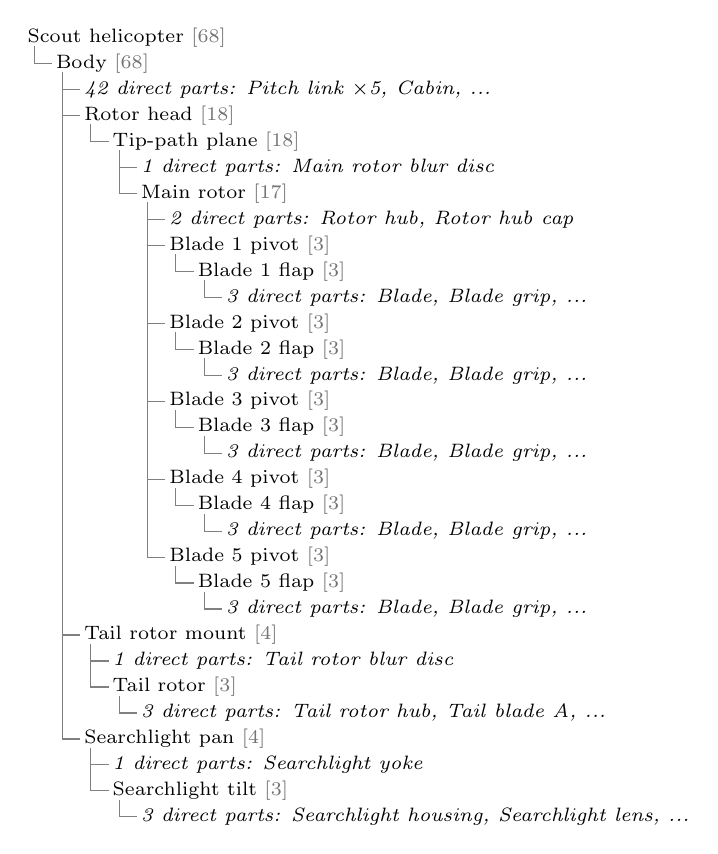
\begin{tikzpicture}[x=0.36cm,y=-0.33cm,font=\scriptsize]
\node[anchor=west,inner sep=0pt] (n0) at (0,0) {Scout helicopter \textcolor{black!55}{[68]}};
\node[anchor=west,inner sep=0pt] (n1) at (1,1) {Body \textcolor{black!55}{[68]}};
\draw[black!50,thin] (0.25,0.35) |- (0.88,1);
\node[anchor=west,inner sep=0pt] (n2) at (2,2) {\textit{42 direct parts: Pitch link $\times$5, Cabin, ...}};
\draw[black!50,thin] (1.25,1.35) |- (1.88,2);
\node[anchor=west,inner sep=0pt] (n3) at (2,3) {Rotor head \textcolor{black!55}{[18]}};
\draw[black!50,thin] (1.25,1.35) |- (1.88,3);
\node[anchor=west,inner sep=0pt] (n4) at (3,4) {Tip-path plane \textcolor{black!55}{[18]}};
\draw[black!50,thin] (2.25,3.35) |- (2.88,4);
\node[anchor=west,inner sep=0pt] (n5) at (4,5) {\textit{1 direct parts: Main rotor blur disc}};
\draw[black!50,thin] (3.25,4.35) |- (3.88,5);
\node[anchor=west,inner sep=0pt] (n6) at (4,6) {Main rotor \textcolor{black!55}{[17]}};
\draw[black!50,thin] (3.25,4.35) |- (3.88,6);
\node[anchor=west,inner sep=0pt] (n7) at (5,7) {\textit{2 direct parts: Rotor hub, Rotor hub cap}};
\draw[black!50,thin] (4.25,6.35) |- (4.88,7);
\node[anchor=west,inner sep=0pt] (n8) at (5,8) {Blade 1 pivot \textcolor{black!55}{[3]}};
\draw[black!50,thin] (4.25,6.35) |- (4.88,8);
\node[anchor=west,inner sep=0pt] (n9) at (6,9) {Blade 1 flap \textcolor{black!55}{[3]}};
\draw[black!50,thin] (5.25,8.35) |- (5.88,9);
\node[anchor=west,inner sep=0pt] (n10) at (7,10) {\textit{3 direct parts: Blade, Blade grip, ...}};
\draw[black!50,thin] (6.25,9.35) |- (6.88,10);
\node[anchor=west,inner sep=0pt] (n11) at (5,11) {Blade 2 pivot \textcolor{black!55}{[3]}};
\draw[black!50,thin] (4.25,6.35) |- (4.88,11);
\node[anchor=west,inner sep=0pt] (n12) at (6,12) {Blade 2 flap \textcolor{black!55}{[3]}};
\draw[black!50,thin] (5.25,11.35) |- (5.88,12);
\node[anchor=west,inner sep=0pt] (n13) at (7,13) {\textit{3 direct parts: Blade, Blade grip, ...}};
\draw[black!50,thin] (6.25,12.35) |- (6.88,13);
\node[anchor=west,inner sep=0pt] (n14) at (5,14) {Blade 3 pivot \textcolor{black!55}{[3]}};
\draw[black!50,thin] (4.25,6.35) |- (4.88,14);
\node[anchor=west,inner sep=0pt] (n15) at (6,15) {Blade 3 flap \textcolor{black!55}{[3]}};
\draw[black!50,thin] (5.25,14.35) |- (5.88,15);
\node[anchor=west,inner sep=0pt] (n16) at (7,16) {\textit{3 direct parts: Blade, Blade grip, ...}};
\draw[black!50,thin] (6.25,15.35) |- (6.88,16);
\node[anchor=west,inner sep=0pt] (n17) at (5,17) {Blade 4 pivot \textcolor{black!55}{[3]}};
\draw[black!50,thin] (4.25,6.35) |- (4.88,17);
\node[anchor=west,inner sep=0pt] (n18) at (6,18) {Blade 4 flap \textcolor{black!55}{[3]}};
\draw[black!50,thin] (5.25,17.35) |- (5.88,18);
\node[anchor=west,inner sep=0pt] (n19) at (7,19) {\textit{3 direct parts: Blade, Blade grip, ...}};
\draw[black!50,thin] (6.25,18.35) |- (6.88,19);
\node[anchor=west,inner sep=0pt] (n20) at (5,20) {Blade 5 pivot \textcolor{black!55}{[3]}};
\draw[black!50,thin] (4.25,6.35) |- (4.88,20);
\node[anchor=west,inner sep=0pt] (n21) at (6,21) {Blade 5 flap \textcolor{black!55}{[3]}};
\draw[black!50,thin] (5.25,20.35) |- (5.88,21);
\node[anchor=west,inner sep=0pt] (n22) at (7,22) {\textit{3 direct parts: Blade, Blade grip, ...}};
\draw[black!50,thin] (6.25,21.35) |- (6.88,22);
\node[anchor=west,inner sep=0pt] (n23) at (2,23) {Tail rotor mount \textcolor{black!55}{[4]}};
\draw[black!50,thin] (1.25,1.35) |- (1.88,23);
\node[anchor=west,inner sep=0pt] (n24) at (3,24) {\textit{1 direct parts: Tail rotor blur disc}};
\draw[black!50,thin] (2.25,23.35) |- (2.88,24);
\node[anchor=west,inner sep=0pt] (n25) at (3,25) {Tail rotor \textcolor{black!55}{[3]}};
\draw[black!50,thin] (2.25,23.35) |- (2.88,25);
\node[anchor=west,inner sep=0pt] (n26) at (4,26) {\textit{3 direct parts: Tail rotor hub, Tail blade A, ...}};
\draw[black!50,thin] (3.25,25.35) |- (3.88,26);
\node[anchor=west,inner sep=0pt] (n27) at (2,27) {Searchlight pan \textcolor{black!55}{[4]}};
\draw[black!50,thin] (1.25,1.35) |- (1.88,27);
\node[anchor=west,inner sep=0pt] (n28) at (3,28) {\textit{1 direct parts: Searchlight yoke}};
\draw[black!50,thin] (2.25,27.35) |- (2.88,28);
\node[anchor=west,inner sep=0pt] (n29) at (3,29) {Searchlight tilt \textcolor{black!55}{[3]}};
\draw[black!50,thin] (2.25,27.35) |- (2.88,29);
\node[anchor=west,inner sep=0pt] (n30) at (4,30) {\textit{3 direct parts: Searchlight housing, Searchlight lens, ...}};
\draw[black!50,thin] (3.25,29.35) |- (3.88,30);
\end{tikzpicture}
\end{minipage}\hfill
\begin{minipage}[t]{0.42\linewidth}\vspace{0pt}% generated by report/gen_tables.py from build/scene_export.json -- do not edit
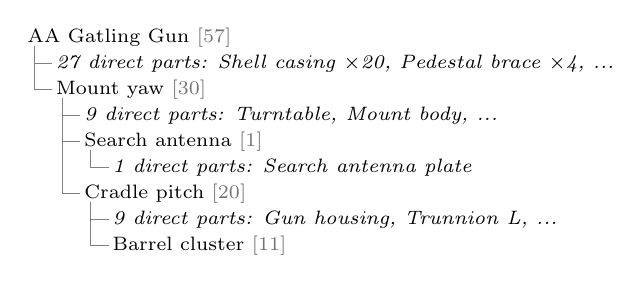
\begin{tikzpicture}[x=0.36cm,y=-0.33cm,font=\scriptsize]
\node[anchor=west,inner sep=0pt] (n0) at (0,0) {AA Gatling Gun \textcolor{black!55}{[57]}};
\node[anchor=west,inner sep=0pt] (n1) at (1,1) {\textit{27 direct parts: Shell casing $\times$20, Pedestal brace $\times$4, ...}};
\draw[black!50,thin] (0.25,0.35) |- (0.88,1);
\node[anchor=west,inner sep=0pt] (n2) at (1,2) {Mount yaw \textcolor{black!55}{[30]}};
\draw[black!50,thin] (0.25,0.35) |- (0.88,2);
\node[anchor=west,inner sep=0pt] (n3) at (2,3) {\textit{9 direct parts: Turntable, Mount body, ...}};
\draw[black!50,thin] (1.25,2.35) |- (1.88,3);
\node[anchor=west,inner sep=0pt] (n4) at (2,4) {Search antenna \textcolor{black!55}{[1]}};
\draw[black!50,thin] (1.25,2.35) |- (1.88,4);
\node[anchor=west,inner sep=0pt] (n5) at (3,5) {\textit{1 direct parts: Search antenna plate}};
\draw[black!50,thin] (2.25,4.35) |- (2.88,5);
\node[anchor=west,inner sep=0pt] (n6) at (2,6) {Cradle pitch \textcolor{black!55}{[20]}};
\draw[black!50,thin] (1.25,2.35) |- (1.88,6);
\node[anchor=west,inner sep=0pt] (n7) at (3,7) {\textit{9 direct parts: Gun housing, Trunnion L, ...}};
\draw[black!50,thin] (2.25,6.35) |- (2.88,7);
\node[anchor=west,inner sep=0pt] (n8) at (3,8) {Barrel cluster \textcolor{black!55}{[11]}};
\draw[black!50,thin] (2.25,6.35) |- (2.88,8);
\end{tikzpicture}
\\[3mm]% generated by report/gen_tables.py from build/scene_export.json -- do not edit
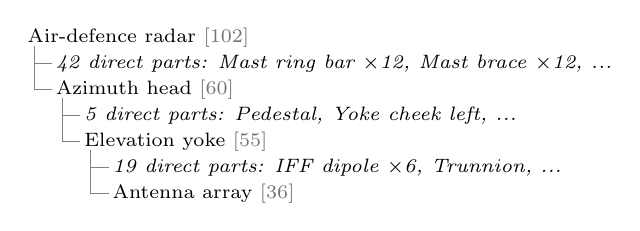
\begin{tikzpicture}[x=0.36cm,y=-0.33cm,font=\scriptsize]
\node[anchor=west,inner sep=0pt] (n0) at (0,0) {Air-defence radar \textcolor{black!55}{[102]}};
\node[anchor=west,inner sep=0pt] (n1) at (1,1) {\textit{42 direct parts: Mast ring bar $\times$12, Mast brace $\times$12, ...}};
\draw[black!50,thin] (0.25,0.35) |- (0.88,1);
\node[anchor=west,inner sep=0pt] (n2) at (1,2) {Azimuth head \textcolor{black!55}{[60]}};
\draw[black!50,thin] (0.25,0.35) |- (0.88,2);
\node[anchor=west,inner sep=0pt] (n3) at (2,3) {\textit{5 direct parts: Pedestal, Yoke cheek left, ...}};
\draw[black!50,thin] (1.25,2.35) |- (1.88,3);
\node[anchor=west,inner sep=0pt] (n4) at (2,4) {Elevation yoke \textcolor{black!55}{[55]}};
\draw[black!50,thin] (1.25,2.35) |- (1.88,4);
\node[anchor=west,inner sep=0pt] (n5) at (3,5) {\textit{19 direct parts: IFF dipole $\times$6, Trunnion, ...}};
\draw[black!50,thin] (2.25,4.35) |- (2.88,5);
\node[anchor=west,inner sep=0pt] (n6) at (3,6) {Antenna array \textcolor{black!55}{[36]}};
\draw[black!50,thin] (2.25,4.35) |- (2.88,6);
\end{tikzpicture}
\end{minipage}
\caption{Hierarchies of the helicopter (left; the tip-path-plane node tilts with the cyclic and each blade flaps and feathers under its own \emph{Blade $i$ flap} node), the AA gun and
the radar (right), from the export. Captures of the same machines are in Fig.~\ref{fig:machines}.}
\label{fig:tree-air}
\end{figure}

% ---------------------------------------------------------------------
\subsection{Gate barrier, windsock and flag}
Three animated objects of the base: the \emph{boom barrier} at the outer gate (\partsBarrier{} parts: boom with five red and five white stripes,
foundation, housing with door, cradle, counterweight on an arm, pivot bolt, tip lamp and warning lamp), the \emph{windsock} (\partsWindsock{} parts: pole, swivel and five chained
segments) and the \emph{flag} (\partsFlag{} parts: pole, fittings and a flag of 12 chained strips). The barrier is possessable; the windsock and flag are animated scenery driven by one shared
wind function.

\begin{figure}[h]
\centering
\begin{minipage}[t]{0.32\linewidth}\vspace{0pt}% generated by report/gen_tables.py from build/scene_export.json -- do not edit
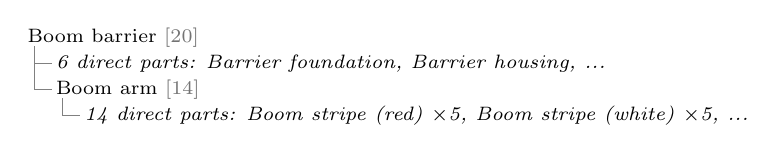
\begin{tikzpicture}[x=0.36cm,y=-0.33cm,font=\scriptsize]
\node[anchor=west,inner sep=0pt] (n0) at (0,0) {Boom barrier \textcolor{black!55}{[20]}};
\node[anchor=west,inner sep=0pt] (n1) at (1,1) {\textit{6 direct parts: Barrier foundation, Barrier housing, ...}};
\draw[black!50,thin] (0.25,0.35) |- (0.88,1);
\node[anchor=west,inner sep=0pt] (n2) at (1,2) {Boom arm \textcolor{black!55}{[14]}};
\draw[black!50,thin] (0.25,0.35) |- (0.88,2);
\node[anchor=west,inner sep=0pt] (n3) at (2,3) {\textit{14 direct parts: Boom stripe (red) $\times$5, Boom stripe (white) $\times$5, ...}};
\draw[black!50,thin] (1.25,2.35) |- (1.88,3);
\end{tikzpicture}
\end{minipage}\hfill
\begin{minipage}[t]{0.32\linewidth}\vspace{0pt}% generated by report/gen_tables.py from build/scene_export.json -- do not edit
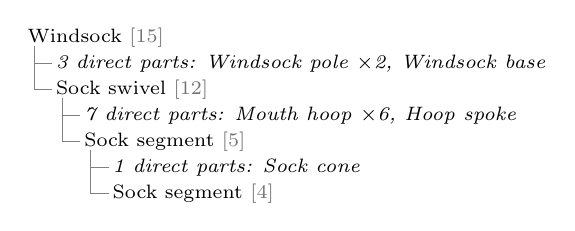
\begin{tikzpicture}[x=0.36cm,y=-0.33cm,font=\scriptsize]
\node[anchor=west,inner sep=0pt] (n0) at (0,0) {Windsock \textcolor{black!55}{[15]}};
\node[anchor=west,inner sep=0pt] (n1) at (1,1) {\textit{3 direct parts: Windsock pole $\times$2, Windsock base}};
\draw[black!50,thin] (0.25,0.35) |- (0.88,1);
\node[anchor=west,inner sep=0pt] (n2) at (1,2) {Sock swivel \textcolor{black!55}{[12]}};
\draw[black!50,thin] (0.25,0.35) |- (0.88,2);
\node[anchor=west,inner sep=0pt] (n3) at (2,3) {\textit{7 direct parts: Mouth hoop $\times$6, Hoop spoke}};
\draw[black!50,thin] (1.25,2.35) |- (1.88,3);
\node[anchor=west,inner sep=0pt] (n4) at (2,4) {Sock segment \textcolor{black!55}{[5]}};
\draw[black!50,thin] (1.25,2.35) |- (1.88,4);
\node[anchor=west,inner sep=0pt] (n5) at (3,5) {\textit{1 direct parts: Sock cone}};
\draw[black!50,thin] (2.25,4.35) |- (2.88,5);
\node[anchor=west,inner sep=0pt] (n6) at (3,6) {Sock segment \textcolor{black!55}{[4]}};
\draw[black!50,thin] (2.25,4.35) |- (2.88,6);
\end{tikzpicture}
\end{minipage}\hfill
\begin{minipage}[t]{0.32\linewidth}\vspace{0pt}% generated by report/gen_tables.py from build/scene_export.json -- do not edit
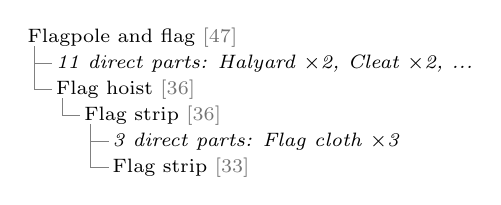
\begin{tikzpicture}[x=0.36cm,y=-0.33cm,font=\scriptsize]
\node[anchor=west,inner sep=0pt] (n0) at (0,0) {Flagpole and flag \textcolor{black!55}{[47]}};
\node[anchor=west,inner sep=0pt] (n1) at (1,1) {\textit{11 direct parts: Halyard $\times$2, Cleat $\times$2, ...}};
\draw[black!50,thin] (0.25,0.35) |- (0.88,1);
\node[anchor=west,inner sep=0pt] (n2) at (1,2) {Flag hoist \textcolor{black!55}{[36]}};
\draw[black!50,thin] (0.25,0.35) |- (0.88,2);
\node[anchor=west,inner sep=0pt] (n3) at (2,3) {Flag strip \textcolor{black!55}{[36]}};
\draw[black!50,thin] (1.25,2.35) |- (1.88,3);
\node[anchor=west,inner sep=0pt] (n4) at (3,4) {\textit{3 direct parts: Flag cloth $\times$3}};
\draw[black!50,thin] (2.25,3.35) |- (2.88,4);
\node[anchor=west,inner sep=0pt] (n5) at (3,5) {Flag strip \textcolor{black!55}{[33]}};
\draw[black!50,thin] (2.25,3.35) |- (2.88,5);
\end{tikzpicture}
\end{minipage}
\caption{Hierarchies of the boom barrier, the windsock and the flag (export). The windsock and the flag are chains in
which every segment is the child of the previous one.}
\end{figure}

% ---------------------------------------------------------------------
\subsection{Environment, terrain and backdrop}
The Gouraud environment (\partsEnv{} parts, grown from 621 in v3) keeps the v3 compound (perimeter fence with wires and gate,
watchtower with floodlight, sandbag walls, camouflaged tent, supply caches, radio mast, lamp posts, fire barrel,
spruces made of cone whorls, broadleaf trees of sphere clumps, bushes and boulders) and adds \emph{military dressing}
(HESCO blocks, a jersey chicane, a sandbag fighting position, a track sign). The trench strip and the bunker
footprint are cleared of vegetation (T78). The terrain is one 36\,m disc of 130 rings $\times$ 384 slices (49\,921
vertices, 97\,440 triangles, a hole for the entrance trench, T13/T61) whose height field has a levelled bunker pad,
a creek, a vehicle track, a berm and a raised mound that keeps at least 0.15\,m of earth above the bunker roof (T60). The backdrop (\partsBackdrop{} parts:
distant hills, a 46-pine tree line at 38--45\,m, a far radio tower at 100\,m) starts beyond the terrain mesh (T79:
nearest part 38.0\,m).

\begin{figure}[h]
\centering
\begin{minipage}[t]{0.6\linewidth}\vspace{0pt}% generated by report/gen_tables.py from build/scene_export.json -- do not edit
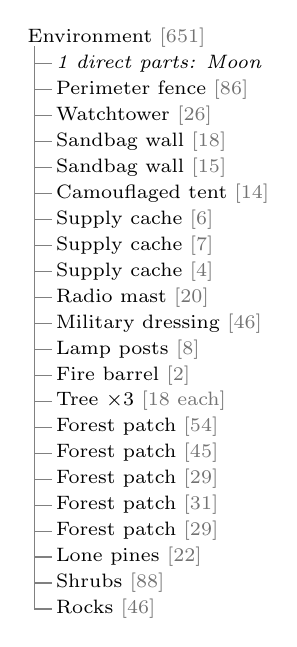
\begin{tikzpicture}[x=0.36cm,y=-0.33cm,font=\scriptsize]
\node[anchor=west,inner sep=0pt] (n0) at (0,0) {Environment \textcolor{black!55}{[651]}};
\node[anchor=west,inner sep=0pt] (n1) at (1,1) {\textit{1 direct parts: Moon}};
\draw[black!50,thin] (0.25,0.35) |- (0.88,1);
\node[anchor=west,inner sep=0pt] (n2) at (1,2) {Perimeter fence \textcolor{black!55}{[86]}};
\draw[black!50,thin] (0.25,0.35) |- (0.88,2);
\node[anchor=west,inner sep=0pt] (n3) at (1,3) {Watchtower \textcolor{black!55}{[26]}};
\draw[black!50,thin] (0.25,0.35) |- (0.88,3);
\node[anchor=west,inner sep=0pt] (n4) at (1,4) {Sandbag wall \textcolor{black!55}{[18]}};
\draw[black!50,thin] (0.25,0.35) |- (0.88,4);
\node[anchor=west,inner sep=0pt] (n5) at (1,5) {Sandbag wall \textcolor{black!55}{[15]}};
\draw[black!50,thin] (0.25,0.35) |- (0.88,5);
\node[anchor=west,inner sep=0pt] (n6) at (1,6) {Camouflaged tent \textcolor{black!55}{[14]}};
\draw[black!50,thin] (0.25,0.35) |- (0.88,6);
\node[anchor=west,inner sep=0pt] (n7) at (1,7) {Supply cache \textcolor{black!55}{[6]}};
\draw[black!50,thin] (0.25,0.35) |- (0.88,7);
\node[anchor=west,inner sep=0pt] (n8) at (1,8) {Supply cache \textcolor{black!55}{[7]}};
\draw[black!50,thin] (0.25,0.35) |- (0.88,8);
\node[anchor=west,inner sep=0pt] (n9) at (1,9) {Supply cache \textcolor{black!55}{[4]}};
\draw[black!50,thin] (0.25,0.35) |- (0.88,9);
\node[anchor=west,inner sep=0pt] (n10) at (1,10) {Radio mast \textcolor{black!55}{[20]}};
\draw[black!50,thin] (0.25,0.35) |- (0.88,10);
\node[anchor=west,inner sep=0pt] (n11) at (1,11) {Military dressing \textcolor{black!55}{[46]}};
\draw[black!50,thin] (0.25,0.35) |- (0.88,11);
\node[anchor=west,inner sep=0pt] (n12) at (1,12) {Lamp posts \textcolor{black!55}{[8]}};
\draw[black!50,thin] (0.25,0.35) |- (0.88,12);
\node[anchor=west,inner sep=0pt] (n13) at (1,13) {Fire barrel \textcolor{black!55}{[2]}};
\draw[black!50,thin] (0.25,0.35) |- (0.88,13);
\node[anchor=west,inner sep=0pt] (n14) at (1,14) {Tree $\times$3 \textcolor{black!55}{[18 each]}};
\draw[black!50,thin] (0.25,0.35) |- (0.88,14);
\node[anchor=west,inner sep=0pt] (n15) at (1,15) {Forest patch \textcolor{black!55}{[54]}};
\draw[black!50,thin] (0.25,0.35) |- (0.88,15);
\node[anchor=west,inner sep=0pt] (n16) at (1,16) {Forest patch \textcolor{black!55}{[45]}};
\draw[black!50,thin] (0.25,0.35) |- (0.88,16);
\node[anchor=west,inner sep=0pt] (n17) at (1,17) {Forest patch \textcolor{black!55}{[29]}};
\draw[black!50,thin] (0.25,0.35) |- (0.88,17);
\node[anchor=west,inner sep=0pt] (n18) at (1,18) {Forest patch \textcolor{black!55}{[31]}};
\draw[black!50,thin] (0.25,0.35) |- (0.88,18);
\node[anchor=west,inner sep=0pt] (n19) at (1,19) {Forest patch \textcolor{black!55}{[29]}};
\draw[black!50,thin] (0.25,0.35) |- (0.88,19);
\node[anchor=west,inner sep=0pt] (n20) at (1,20) {Lone pines \textcolor{black!55}{[22]}};
\draw[black!50,thin] (0.25,0.35) |- (0.88,20);
\node[anchor=west,inner sep=0pt] (n21) at (1,21) {Shrubs \textcolor{black!55}{[88]}};
\draw[black!50,thin] (0.25,0.35) |- (0.88,21);
\node[anchor=west,inner sep=0pt] (n22) at (1,22) {Rocks \textcolor{black!55}{[46]}};
\draw[black!50,thin] (0.25,0.35) |- (0.88,22);
\end{tikzpicture}
\end{minipage}\hfill
\begin{minipage}[t]{0.36\linewidth}\vspace{0pt}\footnotesize
\begin{tabular}{@{}ll@{}}\toprule
Terrain mesh & 130 $\times$ 384, $r=36$\,m\\
Creek depth & $-0.41$\,m (T42)\\
Berm & $+0.44$\,m (T42)\\
Apron level & $-0.30$\,m\\
Far ground top & $-0.35$\,m (T43)\\\bottomrule
\end{tabular}
\end{minipage}
\caption{Environment groups (export, depth 1) and terrain values measured by T42/T43.}
\end{figure}
